\documentclass[aspectratio=169]{beamer}
\setbeamertemplate{navigation symbols}{}
\usepackage{color,amsmath,comment, subfigure}
\usepackage{booktabs}
\usepackage{url}

%%%%%%%%%%%%%%%%%%%%%%%%%%
\title[]{Introduction}
\author[]{Matthew J. Salganik}
\institute[]{Social Network (Soc 204)\\Spring 2021\\Princeton University}
\date[]{Week 1, Lecture 1\\ 2/2: Class structure

\vfill
\begin{flushleft}
\vspace{0.7in}

\includegraphics[width=0.05\textwidth]{figures/cc.png}
\end{flushleft}
}

\begin{document}
%%%%%%%%%%%%%%%%%%%%%%%%%%%
\frame{\titlepage}
%%%%%%%%%%%%%%%%%%%%%%%%%%%
\begin{frame}

\begin{center}
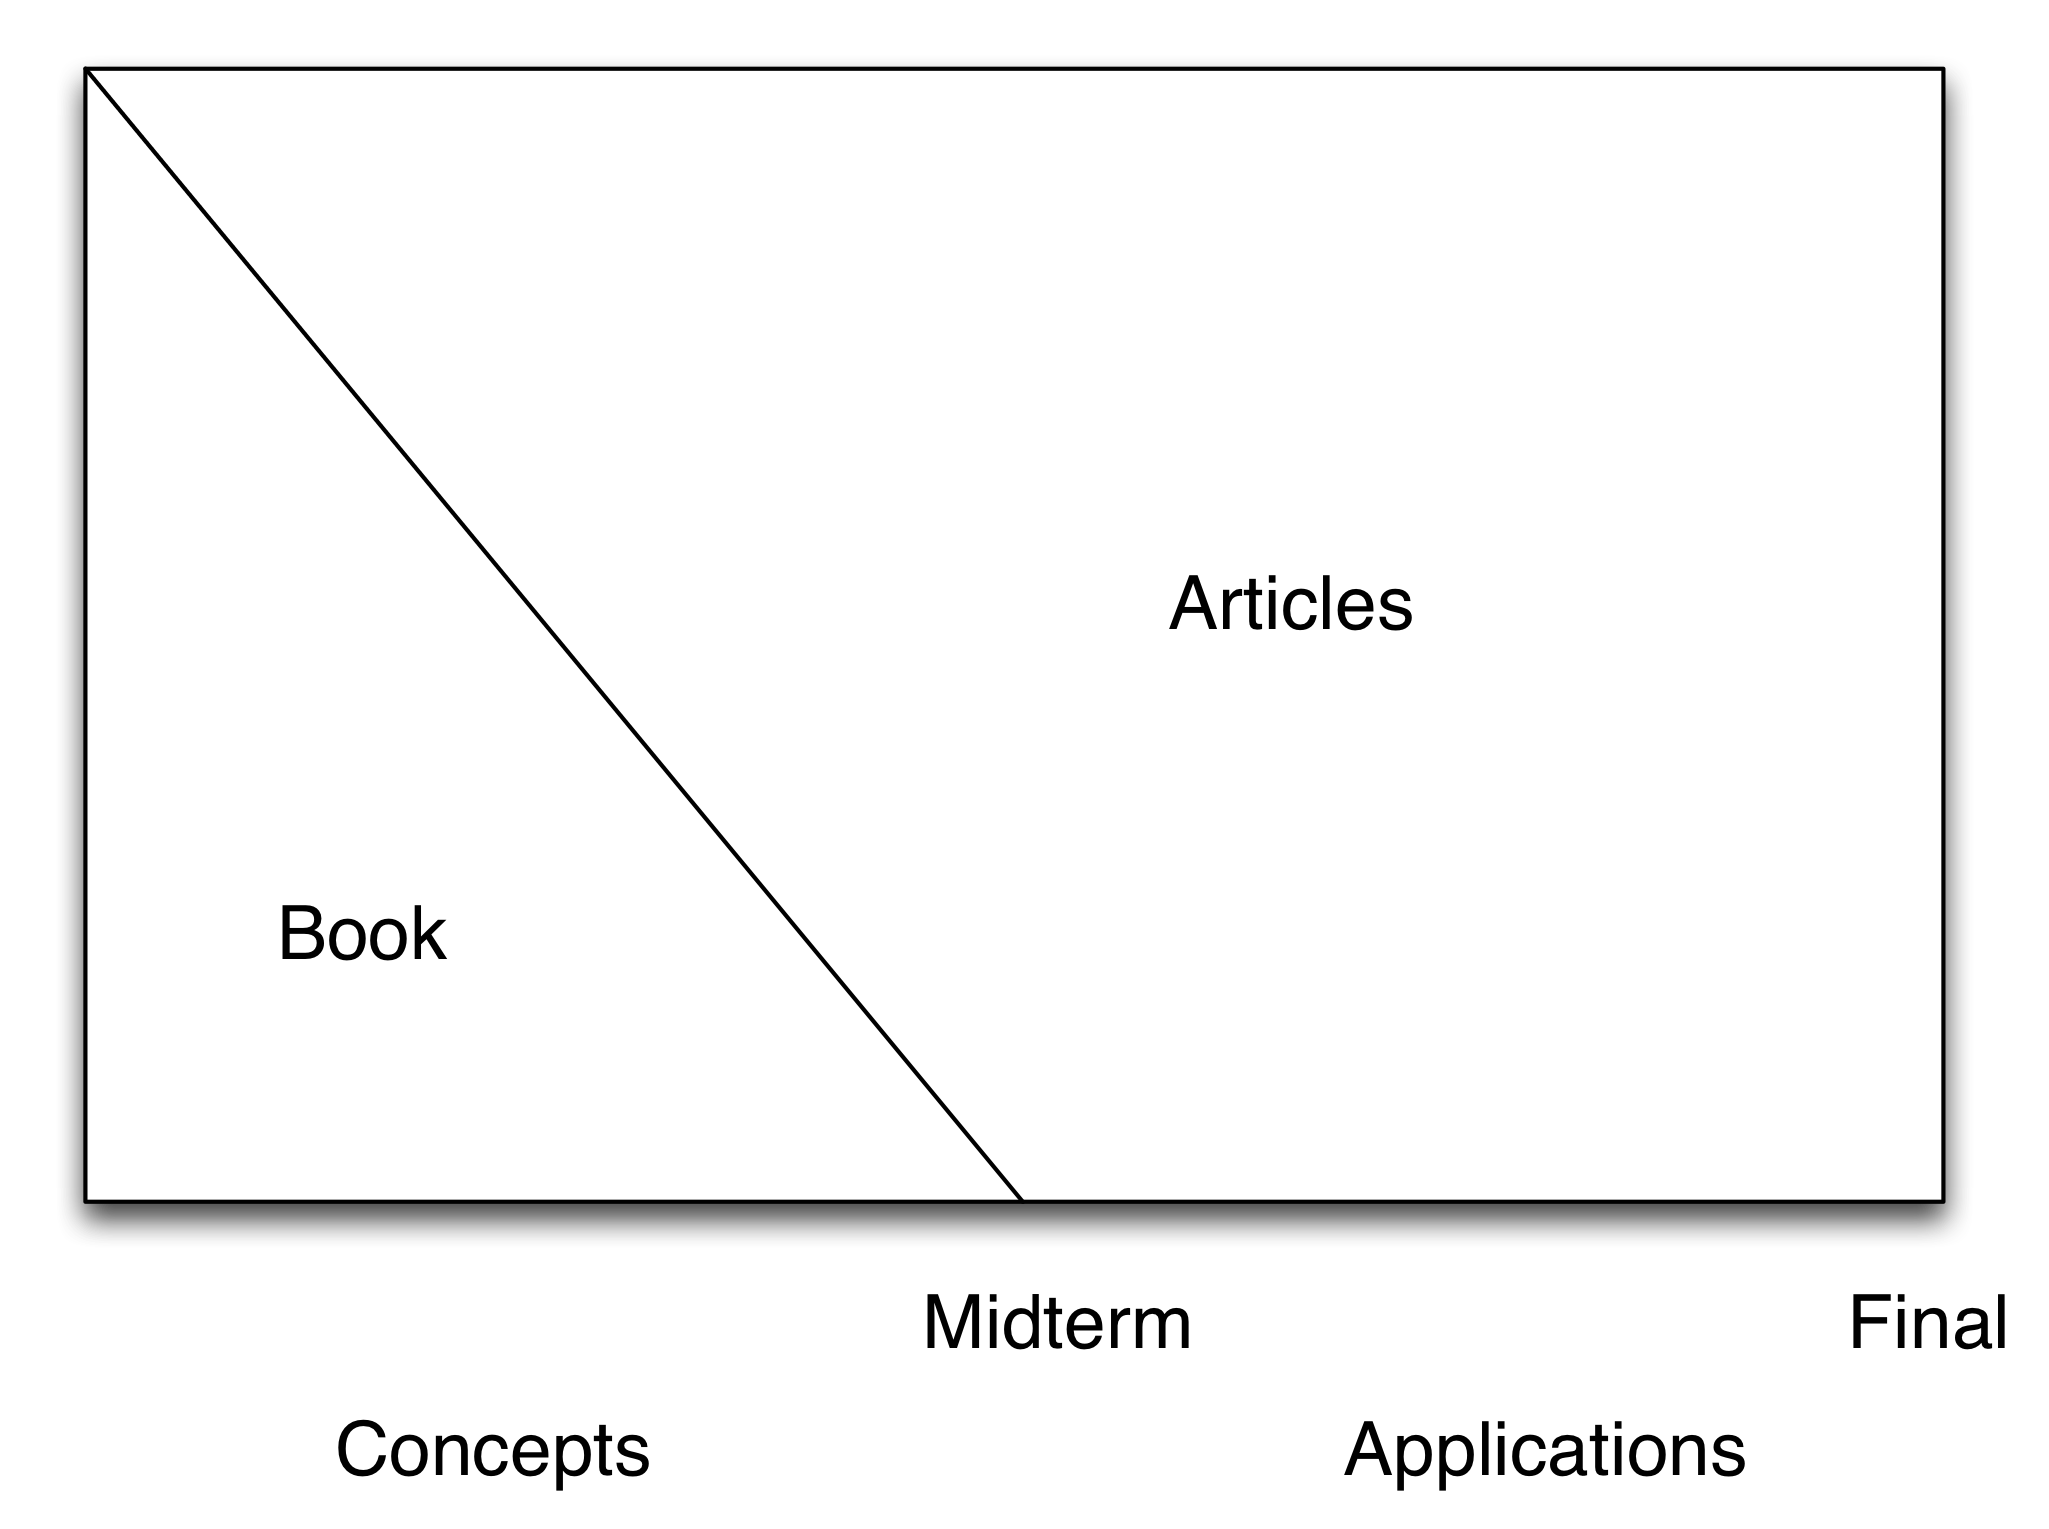
\includegraphics[height=0.90\textheight]{figures/class_structure}
\end{center}

\note{
Not a thriller move that leads up to one big climax, more like a corkscrew that winds around
}

\end{frame}
%%%%%%%%%%%%%%%%%%%%%%%%%%%
\begin{frame}

\begin{itemize}
\item Weekly precept assignment
\item Weekly quiz
\item Midterm exam
\item Final exam
\end{itemize}

\end{frame}
%%%%%%%%%%%%%%%%%%%%%%%%%%%
\begin{frame}

Each week
\begin{itemize}
\item Watch pre-read video
\pause
\item Do reading
\pause
\item Watch pre-recorded lecture video
\pause
\item Watch pre-read video
\item Do reading
\item Watch pre-recorded lecture video 
\pause
\item Take quiz on Canvas
\item Complete weekly assignment
\item Attend precept
\end{itemize}

\end{frame}
%%%%%%%%%%%%%%%%%%%%%%%%%%%%
\begin{frame}

\begin{center}
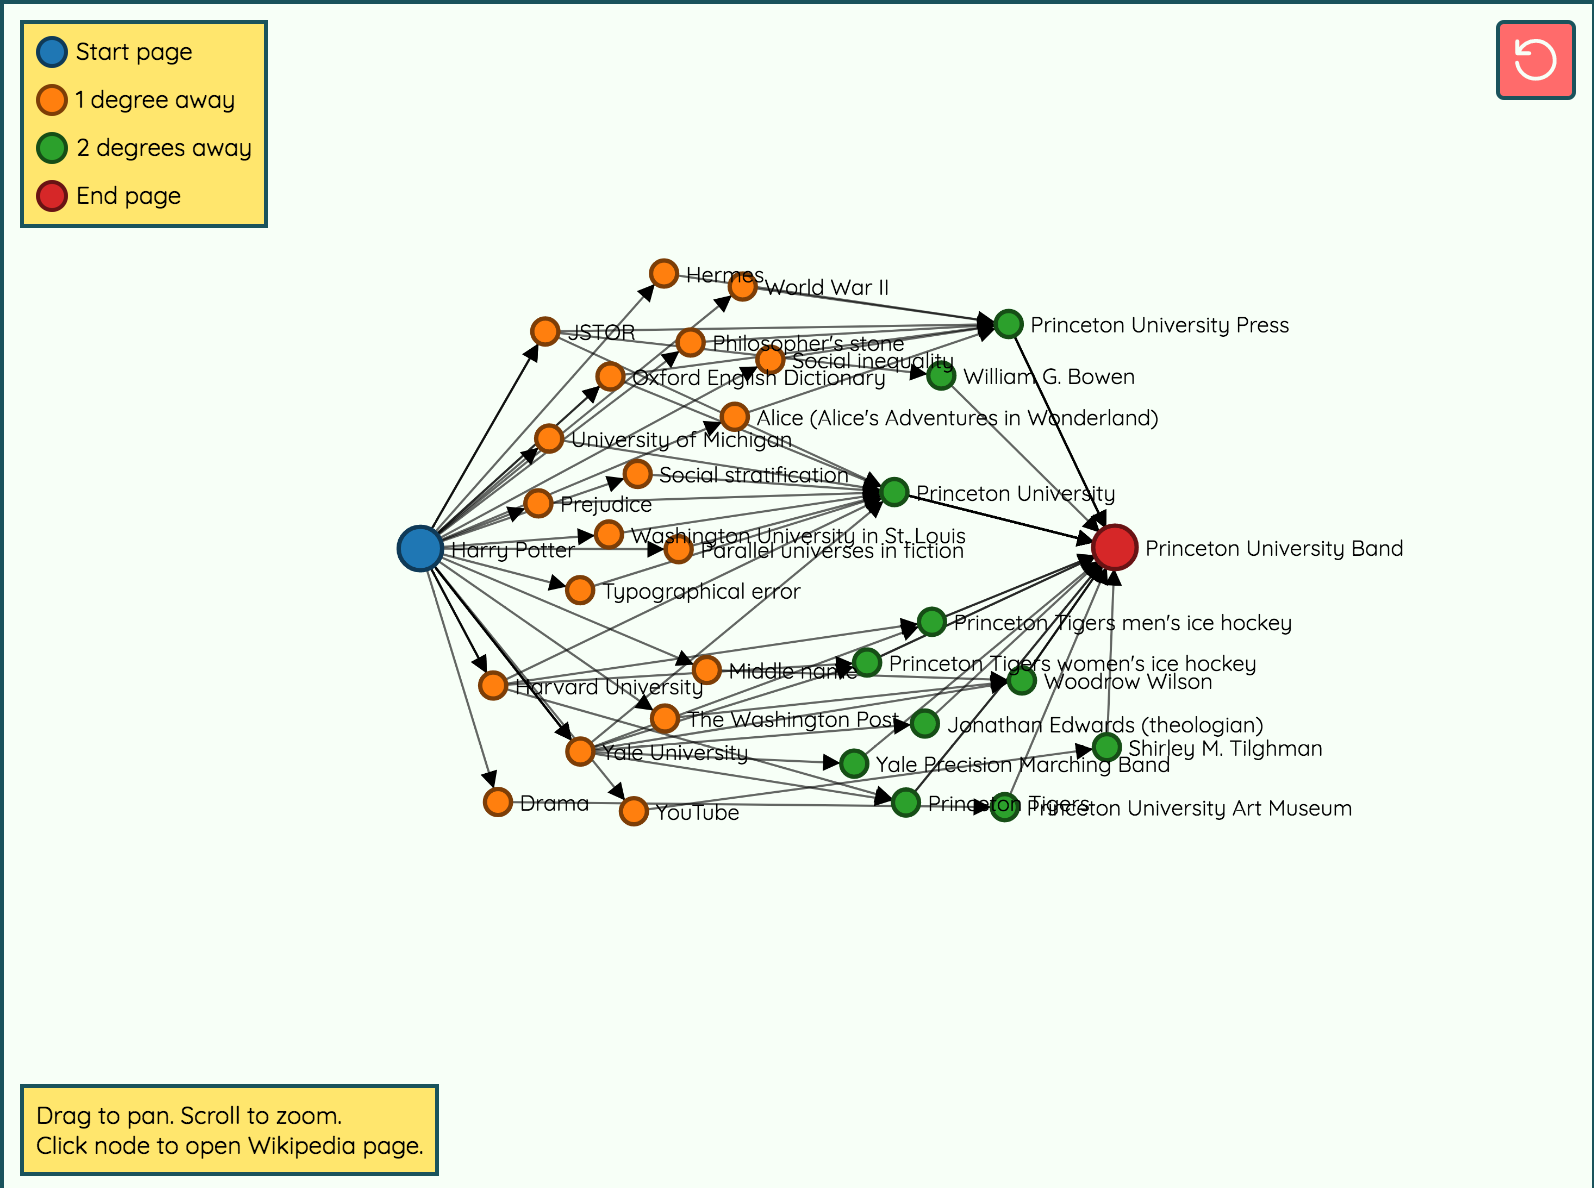
\includegraphics[height=0.9\textheight]{figures/six_degrees_wikipedia_example}
\end{center}

\vfill
\Tiny{\url{https://www.sixdegreesofwikipedia.com/?source=Harry\%20Potter&target=Princeton\%20University\%20Band}}

\end{frame}
%%%%%%%%%%%%%%%%%%%%%%%%%%%
\begin{frame}

\begin{center}

\includegraphics[width=0.95\textwidth]{figures/kramer_experimental_2014_title}
\end{center}

\vfill
\Tiny{\url{https://doi.org/10.1073/pnas.1320040111}}

\end{frame}
%%%%%%%%%%%%%%%%%%%%%%%%%%%
\begin{frame}

\begin{center}

\includegraphics[height=0.90\textheight]{figures/princeton_precept}
\end{center}

\vfill
\Tiny{\url{http://www.princeton.edu/pr/pub/precept/PU-Inspired-Conversations-2008.pdf}}

\note{
Precepts started in 1905
Precept is a time for active learning
You can of course use this time to ask questions, but you should expect to learn new things not just hear a rehash of the lecture
}

\end{frame}
%%%%%%%%%%%%%%%%%%%%%%%%%%%
\begin{frame}

\begin{center}
\Large{Is this course right for you?}
\end{center}

\note{
Working hard, weekly assignments, difficult reading
Support you need to be successful
If you are a senior and you want to focus on thesis this might not be a good class for you
For students in social science and humanities more mathematical, different reading
For computer science engineering students, more reading, different reading
}

\end{frame}
%%%%%%%%%%%%%%%%%%%%%%%%%%%
\begin{frame}

\begin{itemize}
\item Canvas: {\tiny \url{https://princeton.instructure.com/courses/2747}}
\pause
\item Additional information about readings: {\tiny \url{https://www.princeton.edu/~mjs3/soc204_s2021/readings.shtml}}
\pause
\item Additional information about class logistics: {\tiny \url{https://www.princeton.edu/~mjs3/soc204_s2021/logistics.shtml}}
\end{itemize}

\note{
I expect you to read syllabus
}

\end{frame}
%%%%%%%%%%%%%%%%%%%%%%%%%%%%
\begin{frame}

\begin{center}
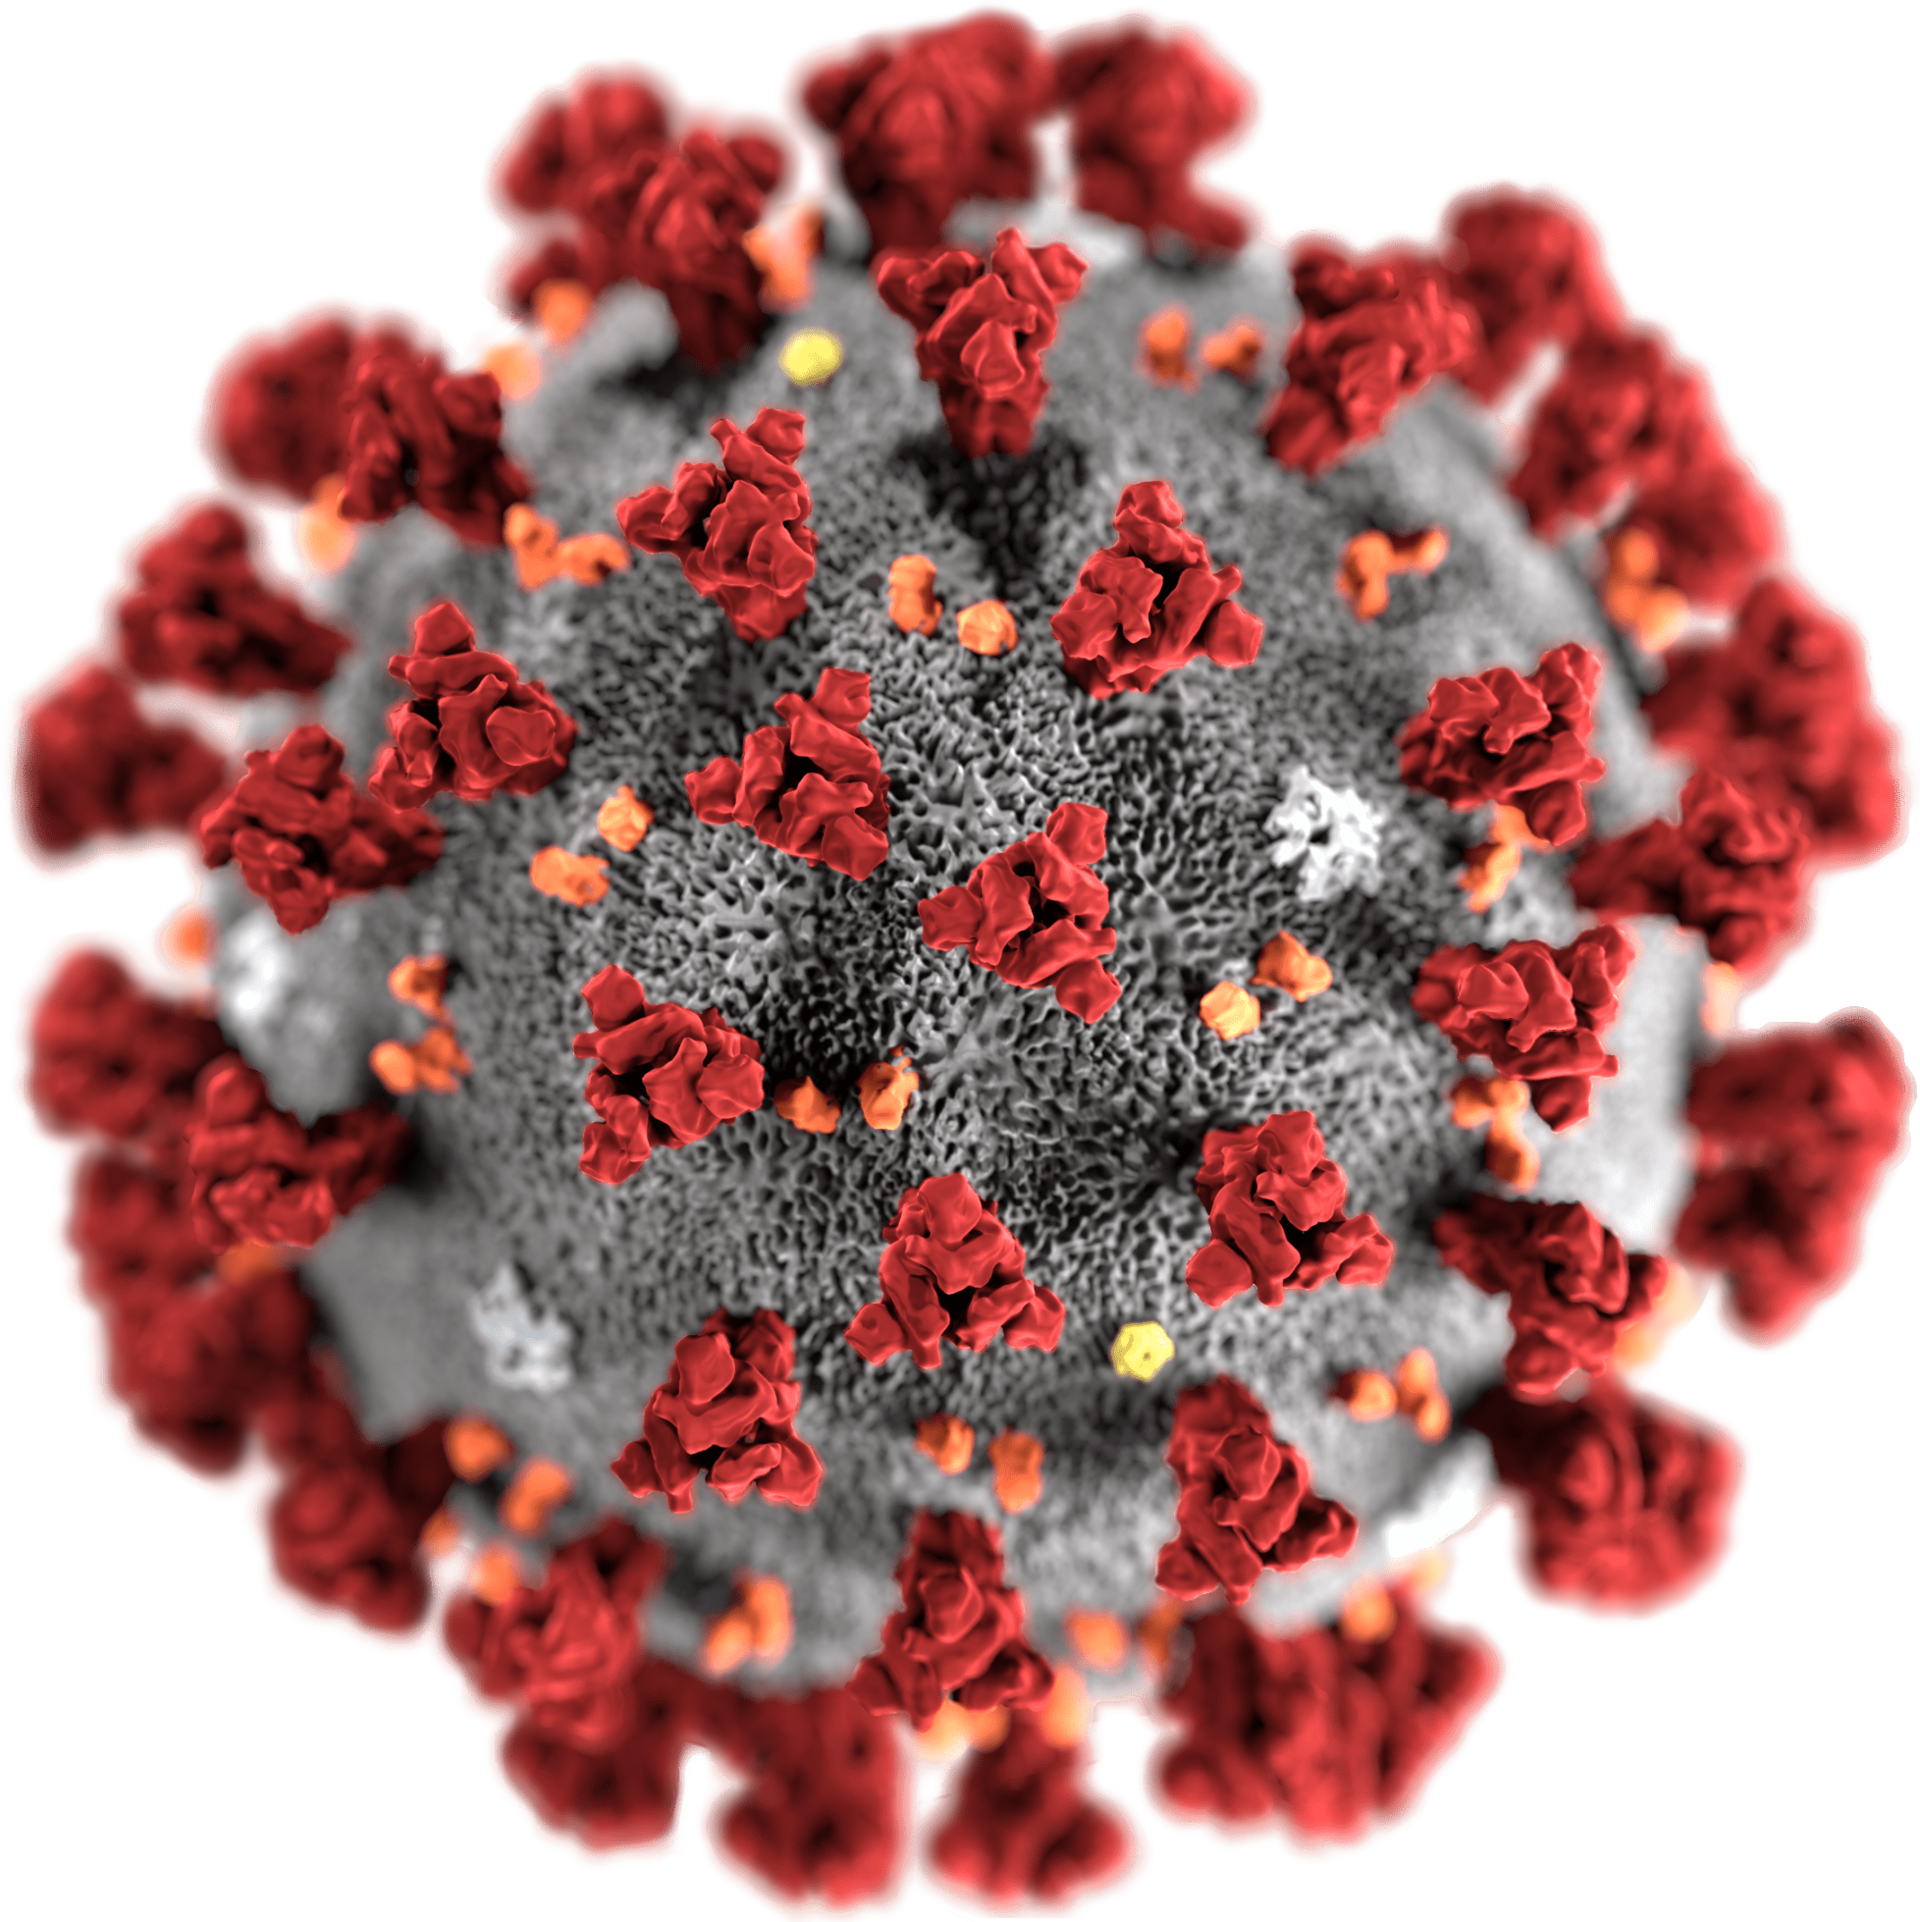
\includegraphics[height = 0.9\textheight]{figures/covid}
\end{center}

\vfill
\tiny{\url{https://phil.cdc.gov/Details.aspx?pid=23312}}

\note{
COVID, hard time for me and my family, first time I'm teaching like this
I'll be asking for feedback a lot to help adjust
If you are having trouble physically or mentally or technologically support is available.
}

\end{frame}
%%%%%%%%%%%%%%%%%%%%%%%%%%%%
\begin{frame}

Next class: The connected age and the small world problem

\end{frame}
%%%%%%%%%%%%%%%%%%%%%%%%%%%


\end{document}
